% Copyright 2016 - 2017 Bas van Meerten and Wouter Franssen
%
%This file is part of ssNake.
%
%ssNake is free software: you can redistribute it and/or modify
%it under the terms of the GNU General Public License as published by
%the Free Software Foundation, either version 3 of the License, or
%(at your option) any later version.
%
%ssNake is distributed in the hope that it will be useful,
%but WITHOUT ANY WARRANTY; without even the implied warranty of
%MERCHANTABILITY or FITNESS FOR A PARTICULAR PURPOSE.  See the
%GNU General Public License for more details.
%
%You should have received a copy of the GNU General Public License
%along with ssNake. If not, see <http://www.gnu.org/licenses/>.

\documentclass[11pt,a4paper]{article}
% Copyright 2016 - 2017 Bas van Meerten and Wouter Franssen
%
%This file is part of ssNake.
%
%ssNake is free software: you can redistribute it and/or modify
%it under the terms of the GNU General Public License as published by
%the Free Software Foundation, either version 3 of the License, or
%(at your option) any later version.
%
%ssNake is distributed in the hope that it will be useful,
%but WITHOUT ANY WARRANTY; without even the implied warranty of
%MERCHANTABILITY or FITNESS FOR A PARTICULAR PURPOSE.  See the
%GNU General Public License for more details.
%
%You should have received a copy of the GNU General Public License
%along with ssNake. If not, see <http://www.gnu.org/licenses/>.

\usepackage[british]{babel}
\usepackage{graphicx,booktabs,listings,amsmath,pgfplots,pgfplotstable}
\usepackage[small,bf,nooneline]{caption}
\usepackage{subcaption}
\usepackage[sort&compress,numbers]{natbib}
\usepackage{tikz}
\usepackage{mathtools}
\usepackage[nottoc]{tocbibind}%adds bibliography to table of contents.
\graphicspath{{./images/}}
%\setlength{\textwidth}{453pt} %597 pt is the a4 paperwidth. Minus 2 in margin. 72 pt = 1 in
%\setlength{\hoffset}{-\oddsidemargin}
%\setlength{\voffset}{-30pt} %
%\setlength{\textheight}{651 pt} %a4 height 845 pt minus 2* total headheight. In this case 2*88pt
%% examine margines via the layout package. Use command \layout{} in document to draw a picture.
%\setlength{\parindent}{0.5 cm}
%\setlength{\parskip}{0 cm}
\usepackage[left=82pt,right=82pt,top=95pt,bottom=95pt,footnotesep=0.5cm]{geometry}
%\setlength{\headheight}{14pt}

%define colours--------------------
%dark
\usepackage{xcolor}
\definecolor{MyGrayD}{RGB}{1,1,1}
\definecolor{MyRedD}{RGB}{237,45,46}
\definecolor{MyGreenD}{RGB}{0,140,71}
\definecolor{MyBlueD}{RGB}{24,89,169}
\definecolor{MyOrangeD}{RGB}{243,125,34}
\definecolor{MyPurpleD}{RGB}{102,44,145}
\definecolor{MyBrownD}{RGB}{161,29,32}
\definecolor{MyPinkD}{RGB}{179,56,147}
%normal
\definecolor{MyGray}{RGB}{114,114,114}
\definecolor{MyRed}{RGB}{241,89,95}
\definecolor{MyGreen}{RGB}{121,195,106}
\definecolor{MyBlue}{RGB}{89,154,211}
\definecolor{MyOrange}{RGB}{249,166,90}
\definecolor{MyPurple}{RGB}{158,102,171}
\definecolor{MyBrown}{RGB}{205,112,88}
\definecolor{MyPink}{RGB}{215,127,179}
%light
\definecolor{MyGrayL}{RGB}{204,204,204}
\definecolor{MyRedL}{RGB}{242,174,172}
\definecolor{MyGreenL}{RGB}{216,228,170}
\definecolor{MyBlueL}{RGB}{184,210,235}
\definecolor{MyOrangeL}{RGB}{242,209,176}
\definecolor{MyPurpleL}{RGB}{212,178,211}
\definecolor{MyBrownL}{RGB}{221,184,169}
\definecolor{MyPinkL}{RGB}{235,191,217}
%----------------------------------

%Figure ref with hyperref
\newcommand{\fref}[1]{\hyperref[#1]{Figure \ref*{#1}}}
\newcommand{\sref}[1]{\hyperref[#1]{Section \ref*{#1}}}
\newcommand{\tref}[1]{\hyperref[#1]{Table \ref*{#1}}}

%Makes a new command for figures with input values: filename, width(times linewidth),
% caption and label.
\newcommand{\onefigure}[4]{
\setlength{\captionwidth}{#2\linewidth}
\begin{figure}
\includegraphics[width=#2\linewidth]{#1}
\centering
\parbox{\linewidth}{\caption{#3}
\label{#4}}
\end{figure}
}

%Makes a new command for tikz figures with input values: tikz commands, 
% caption and label.
\newcommand{\onetikz}[3]{
\settowidth{\captionwidth}{#1}
\ifthenelse{\lengthtest{\captionwidth<0.7\linewidth}}{\setlength{\captionwidth}{0.7\linewidth}}{}

\begin{figure}
\centering
#1
\centering
\parbox{\linewidth}{\caption{#2}
\label{#3}}
\end{figure}
}

%Makes a new command for two figures next to each other with input values: filename1, caption1, label1,filename2, caption2 and label2. Figure width is set to 0.47\linewidth and the space between the figures is filled with \hfill so the sides of the figures align with to edge of the line.
\newcommand{\twofigure}[6]{
\setlength{\captionwidth}{\linewidth}
\begin{figure*}[ht!]
\begin{minipage}[t]{0.47\linewidth}
\includegraphics[width=\linewidth]{#1}
\centering
\caption{#2}
\label{#3}
\end{minipage}
\hfill
\begin{minipage}[t]{0.47\linewidth}
\centering
\includegraphics[width= \linewidth]{#4}
\centering
\caption{#5}
\label{#6}
\end{minipage}
\end{figure*}
}


%Makes a new command for a table with caption witdh equal to the total table width. Input: tabular, caption and label. Example:
%\onetable{
%\begin{tabular}{ccc}
%a&b&c\\
%\hline
%1&1&1\\
%1&1&1\\
%1&1&1\\
%\end{tabular}
%{The caption.}
%{tab:table1}
%}
\newcommand{\onetable}[3]{
\settowidth{\captionwidth}{#1}
\ifthenelse{\lengthtest{\captionwidth<0.7\linewidth}}{\setlength{\captionwidth}{0.7\linewidth}}{}
\begin{table}
\caption{#2}
\vspace{-0.24cm} %Puts caption close to toprule
\label{#3}
\centering
#1
\end{table}
}

%Makes a long table with captionwidth equal to tablewidth. It takes the following arguments:
%1: Column specifier (e.g. cccc)
%2: Caption
%3: Label
%4: First head (i.e. first row of regular table)
%5: Head of consecutive pages
%6: Foot of pagebreak
%7: Lastfoot (e.g. \midrule)
%8: Body of table
\newcommand{\onelongtable}[8]{
\begin{center}
\settowidth{\captionwidth}{
\begin{tabular}{#1}
#4
#8
\end{tabular}} % This ends the captionwidth part. Next comes the real table.

\begin{longtable}{#1}
\caption{#2}\\
\vspace{-0.74cm} %Puts caption close to toprule
\label{#3}\\

#4
\endfirsthead

#5
\endhead

#6
\endfoot

#7
\endlastfoot

#8
\end{longtable}
\end{center}}




%1:pgfplots code
%2:width
%3:caption
%4:label
\newcommand{\pgfplotsfigure}[4]{
\pgfplotsset{width=#2\linewidth}
\setlength{\captionwidth}{#2\linewidth}
\begin{figure}[t]
\centering
#1
\centering
\parbox{\linewidth}{\caption{#3}
\label{#4}}
\end{figure}
}


\usepackage[bitstream-charter]{mathdesign}
\usepackage[T1]{fontenc}
\usepackage[protrusion=true,expansion,tracking=true]{microtype}
\pgfplotsset{compat=1.7,/pgf/number format/1000 sep={}, axis lines*=left,axis line style={gray},every outer x axis line/.append style={-stealth'},every outer y axis line/.append style={-stealth'},tick label style={font=\small},label style={font=\small},legend style={font=\footnotesize}}
\usepackage{colortbl}
\usetikzlibrary{calc}

%Set section font
\usepackage{sectsty}
\allsectionsfont{\color{black!70}\fontfamily{SourceSansPro-LF}\selectfont}
%--------------------


%Set toc fonts
\usepackage{tocloft}
%\renewcommand\cftchapfont{\fontfamily{SourceSansPro-LF}\bfseries}
\renewcommand\cfttoctitlefont{\color{black!70}\Huge\fontfamily{SourceSansPro-LF}\bfseries}
\renewcommand\cftsecfont{\fontfamily{SourceSansPro-LF}\selectfont}
%\renewcommand\cftchappagefont{\fontfamily{SourceSansPro-LF}\bfseries}
\renewcommand\cftsecpagefont{\fontfamily{SourceSansPro-LF}\selectfont}
\renewcommand\cftsubsecfont{\fontfamily{SourceSansPro-LF}\selectfont}
\renewcommand\cftsubsecpagefont{\fontfamily{SourceSansPro-LF}\selectfont}
%--------------------

%Define header/foot
\usepackage{fancyhdr}
\pagestyle{fancy}
\fancyhead[LE,RO]{\fontfamily{SourceSansPro-LF}\selectfont \thepage}
\fancyhead[LO,RE]{\fontfamily{SourceSansPro-LF}\selectfont \leftmark}
\fancyfoot[C]{}
%--------------------

%remove page number from first chapter page
\makeatletter
\let\ps@plain\ps@empty
\makeatother
%----------------------
\usepackage{blindtext, color}
\definecolor{gray75}{gray}{0.75}
\newcommand{\hsp}{\hspace{20pt}}



\usepackage[hidelinks,colorlinks,allcolors=black, pdftitle={Whole echo acquisition},pdfauthor={W.M.J.\ Franssen}]{hyperref}

\interfootnotelinepenalty=10000 %prevents splitting of footnote over multiple pages
\linespread{1.2}

%\usepgfplotslibrary{external}%creates all external tikz images that are included.
%\tikzexternalize[shell escape=-enable-write18]%activate externalization
%\tikzsetexternalprefix{GeneratedFigures/}
%\tikzset{external/force remake} %Enable forced remake

\title{\color{black}\fontfamily{SourceSansPro-LF}\bfseries Whole echo acquisition data processing using ssNake}
\date{\color{black}\fontfamily{SourceSansPro-LF}\bfseries \today}


\begin{document}


\def\nucleuswidth{2cm} %Distance from nucleus label to start
\def\exwidth{0.6cm} %width of 90 deg pulse
\def\exheight{2cm} %heigth of 90 deg pulse
\def\inwidth{1cm} %width of 180 pulse
\def\inheigth{1.5cm} %heigth of 180 pulse
\def\tauwidth{3cm} %width of standard delay
\def\arrowsep{0.1cm} %space between the start of an arrow and the actual border
\def\arrowheigth{0.7cm} %height of arrow above baseline
\def\fidlength{2.5} %This variable must be without unit! It is used in the domain part of the echo and fid. Must be the same as \fidlengthCM, which is used in the arrows (for which a unit must be specified)
\def\fidlengthCM{2.5cm} %length of the FID
\def\fidarrowheight{-2cm} %heigth of the errow for the FID label
\def\fidheigth{2 cm} %defines the heigth of the FID and echo
\def\repeatheight{2.5cm} %heigth of the repeatblock
\def\repeatwidth{0.3cm} %width of the repeatblock bracket i.e. [
\def\repeatdepth{2.2cm}
\def\freq{30} %defines the frequency of the FID and echo, 
\def\t2{0.3} %defines the exponential decay of the fid and echo



%ExPulse-----------------------------
%Call with \ExPulse[Label][ArrowLabel]{Arrowheight}
%The arguments in brackets are optional. Use:
%\ExPulse{}  for only pulse
%\ExPulse[$\phi$]{}  for pulse with phase label
%\ExPulse[][$t_1$]{\arrowheight}  for pulse with arrow and label (make label ' ' for arrow without label)
%\ExPulse[$\phi$][$t_1$]{\arrowheight}  for pulse with arrow, label and phase.
\newcommand{\ExPulse}[1][]{%
  \def\Label{#1}%
  \draw [fill=gray] (Position) rectangle ++(\exwidth,\exheight); %draw the rectangle
  \ExPulseNext
}
\newcommand{\ExPulseNext}[2][]{%
\ifx&\Label&%
      %do nothing
\else
     \draw (Position) ++ ($(\exwidth/2,\exheight)$) ++ (0,2ex) node [anchor=base] {\Label};%node above the middle
\fi
\ifx&#1&%
      %do nothing
\else
      \draw [->] ($(Position) + (0,-#2)$) -- + ($(\exwidth,0)$);%draw arrow 
 	 \draw ($(Position) + (\exwidth/2,-#2)$) ++ (0,0ex) node [anchor=north]{#1};%label arrow middle
\fi
\coordinate (Position) at ($(Position)+(\exwidth,0)$);%change position
}
%-------------------------------------------


%InPulse-----------------------------
%Call with \InPulse[Label][ArrowLabel]{Arrowheight}
%The arguments in brackets are optional. Use:
%\InPulse{}  for only pulse
%\InPulse[$\phi$]{}  for pulse with phase label
%\InPulse[][$t_1$]{\arrowheight}  for pulse with arrow and label (make label ' ' for arrow without label)
%\InPulse[$\phi$][$t_1$]{\arrowheight}  for pulse with arrow, label and phase.
\newcommand{\InPulse}[1][]{%
  \def\Label{#1}%
  \draw [fill=gray] (Position) rectangle ++(\inwidth,\inheigth);%draw rectangle
  \InPulseNext
}
\newcommand{\InPulseNext}[2][]{%
\ifx&\Label&%
      %do nothing
\else
     \draw (Position) ++ ($(\inwidth/2,\inheigth)$)++ (0,2ex) node [anchor=base] {\Label};%draw label
\fi

\ifx&#1&%
      %do nothing
\else
      \draw [->] ($(Position) + (0,-#2)$) -- + ($(\inwidth,0)$);%draw arrow 
 	 \draw ($(Position) + (\inwidth/2,-#2)$)++ (0,0) node [anchor=north]{#1};%label arrow middle
\fi
\coordinate (Position) at ($(Position)+(\inwidth,0)$);%change position
}
%-------------------------------------------


%Delay-----------------------------
%call with Delay[arrowheight][label]{}
%If no arrowheight: default
%If no label: no arrow (so \Delay[][ ]{} will draw a arrow at the default with no label (only a space)
\newcommand{\Delay}[1][]{%
\ifx&#1&%
	\def\Height{\arrowheigth}%
\else
	\def\Height{#1}
\fi
  
  \DelayNext
}
\newcommand{\DelayNext}[2][]{%
\ifx&#2&%
	\def\Width{\tauwidth}%
\else
	\def\Width{#2}
\fi

\draw (Position) -- ++(\Width,0); %draw baseline

\ifx&#1&%
      %do nothing
\else
	 \draw [<->] ($(Position) + (\arrowsep,\Height)$) -- + ($(\Width-2*\arrowsep,0)$);%draw arrow
     \draw ($(Position) + (\Width/2,\Height)$) node [shape=rectangle,fill=white,draw=white,draw]{#1}; %draw arrow label
\fi

\coordinate (Position) at ($(Position)+(\Width,0)$);%change position
}
%-------------------------------------------


%FID-----------------------------
\newcommand{\FID}[1][]{%
\ifx&#1&%
	\def\Height{\fidarrowheight}%
\else
	\def\Height{#1}
\fi

%  \draw (Position) -- ++ (\fidlengthCM,0);%draw baseline
  \draw let \p1 = (Position) in [domain=0:\fidlength,smooth,samples=100,xshift=\x1,yshift=\y1] plot (\x,{\fidheigth*cos((\x)*\freq r)*exp(-(\x)/\t2)});%draw fid at the correct position (shifted)
  \FIDNext
 }
\newcommand{\FIDNext}[1][]{%
\ifx&#1&%
      %do nothing
\else
	\draw [->] ($(Position) + (0,\Height)$) -- +($(\fidlengthCM-\arrowsep,0)$);%draw arrow
	\draw ($(Position) + (\fidlengthCM/2,\Height)$) node [anchor=north] {#1};%draw label
\fi

\coordinate (Position) at ($(Position)+(\fidlength,0)$);%change position
}
%---------------------------------

%Echo-----------------------------
\newcommand{\Echo}[1][]{%
\ifx&#1&%
	\def\Height{\fidarrowheight}%
\else
	\def\Height{#1}
\fi

%  \draw (Position) -- ++ ($(2*\fidlengthCM,0)$);%baseline
  \draw let \p1 = ($(Position)+(\fidlengthCM,0)$) in [domain=-\fidlength:\fidlength,smooth,samples=200,xshift=\x1,yshift=\y1] plot (\x,{\fidheigth*cos((\x)*\freq r)*exp(-abs(\x)/\t2)});%echo 
  \EchoNext
}

\newcommand{\EchoNext}[1][]{%
\ifx&#1&%
      %do nothing
\else
	\draw [->] ($(Position) + (0,\Height)$) -- +($(2*\fidlengthCM-\arrowsep,0)$);%arrow
	\draw ($(Position) + (\fidlengthCM,\Height)$) node [anchor=north] {#1};%label
\fi

\coordinate (Position) at ($(Position)+(2*\fidlength,0)$);%change position
}
%---------------------------------

\newcommand{\OpenRepeat}{%opens a repeat block
\draw [semithick] (Position) -- ++ (0,\repeatheight) -- ++ (\repeatwidth,0);
\draw [semithick] (Position) -- ++ (0,-\repeatdepth) -- ++ (\repeatwidth,0);
}

\newcommand{\CloseRepeat}[1]{%closes a repeat block with multiplication label as entry
\draw [semithick] (Position) -- ++ (0,\repeatheight) node [anchor=south west] {#1}-- ++ (-\repeatwidth,0);
\draw [semithick] (Position) -- ++ (0,-\repeatdepth) -- ++ (-\repeatwidth,0);
}

\newcommand{\Nucleus}[1]{%specifies the nucleus type at the beginning of the sequence
\draw (Position) node{\large #1};%draw nucleas symbole
\coordinate (Position) at ($(Position)+(\nucleuswidth,0)$);%change position
}
%\newgeometry{left=72pt,right=72pt,top=95pt,bottom=95pt,footnotesep=0.5cm}
\microtypesetup{protrusion=true} % enables protrusion

\maketitle

\section{Introduction}
In the following, we will explain how to processed a whole echo acquired data set. The tutorial delivered with the ssNake program is considered as prior knowledge. If you have not yet studied this, please do so before continuing with this example.

Whole echo acquisition is a nice trick to make powder patterns easier (and thus more accurate) to phase. NMR signals from powders have the tendency to decay quite rapidly due to destructive interference. Using an echo, the start of the signal can be `delayed ' in such a way that it does not fall in the dead time of the probe, and allows for a proper recording of the signal. Whole echo acquisition means that the recording of the signal is started well before the echo top, in such a way that both the rising and decay of the echo is measured. When processed correctly, the imaginary part of the spectrum goes to zero, and phasing is straightforward.

\section{Used data}
For this example, we will use a Varian data set recorded at 14.1~T. The sample was a fine powder of lanthanum fluoride (LaF$_3$), and the $^{139}$La signal is being measured. The setting were such that the echo top is in the centre of the acquisition period.

\section{Processing}
\begin{itemize}
\item Open the data file by using File $\longrightarrow$ Open (or drag and drop).
\item Put the display on absolute (Abs) via the bottom frame under `Plot:'
\end{itemize}
Setting the view on absolute allows easy identification of the echo top. Now we need to swap the echo and put one part at the start, and one part at the end of the signal. As the signal is symmetric around the echo maximum, this will force the imaginary part of the spectrum to zero.
\begin{itemize}
\item Swap the echo via `Tools $\longrightarrow$ Swap Echo' and left-click on the echo top to set the index (about 468), and press OK. 
\end{itemize}
This will show the following:
\begin{center}
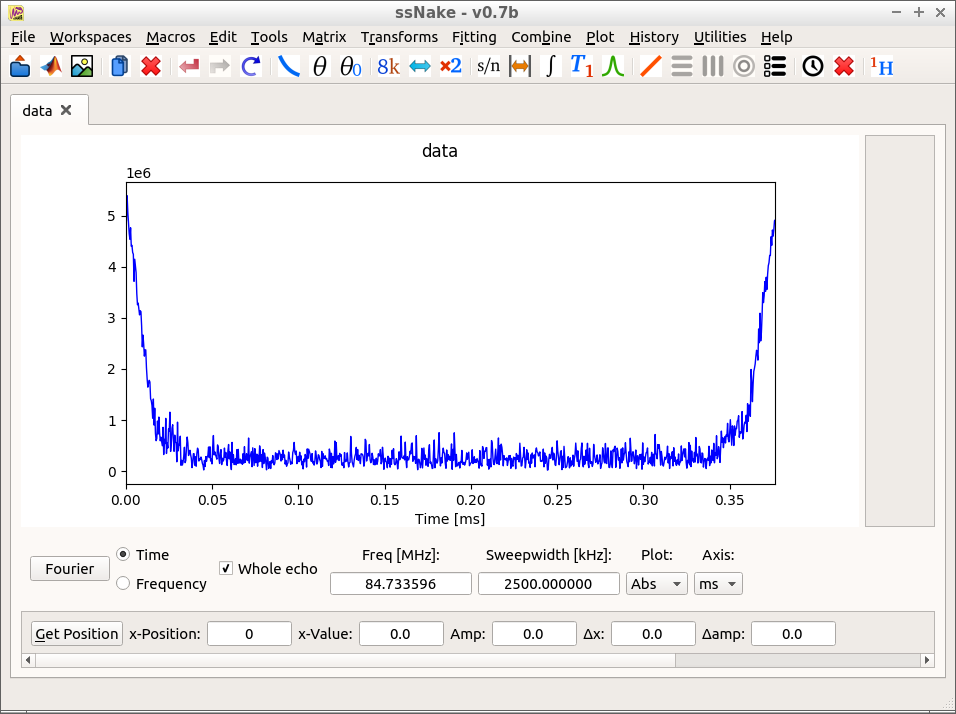
\includegraphics[width=0.8\linewidth]{Figs/Fig1.png}
\end{center}

Note that the `Whole Echo' check box in the bottom frame is now activated. This makes sure that zerofilling is now done at the centre in stead of at the end of the signal. Also, apodizing is done in a symmetric way.
\begin{itemize}
\item Zerofill to `4k' points via `Matrix $\longrightarrow$ Sizing' 
\item Apodize using 1500 Hz Lorentzian broadening (`Tools  $\longrightarrow$ Apodize')
\end{itemize}
This should show the following:
\begin{center}
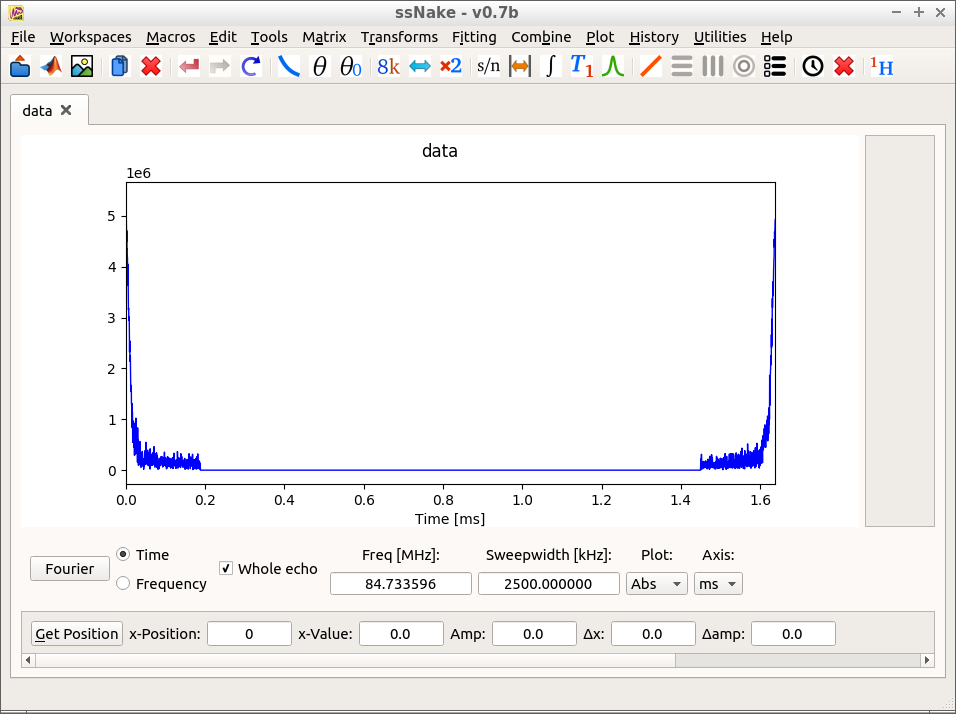
\includegraphics[width=0.8\linewidth]{Figs/Fig2.png}
\end{center}

\begin{itemize}
\item Fourier transform via the `Fourier' button
\item Put the display at `Both' via the bottom frame, to show the real and imaginary part of the spectrum
\end{itemize}
This shows (zoomed in):
\begin{center}
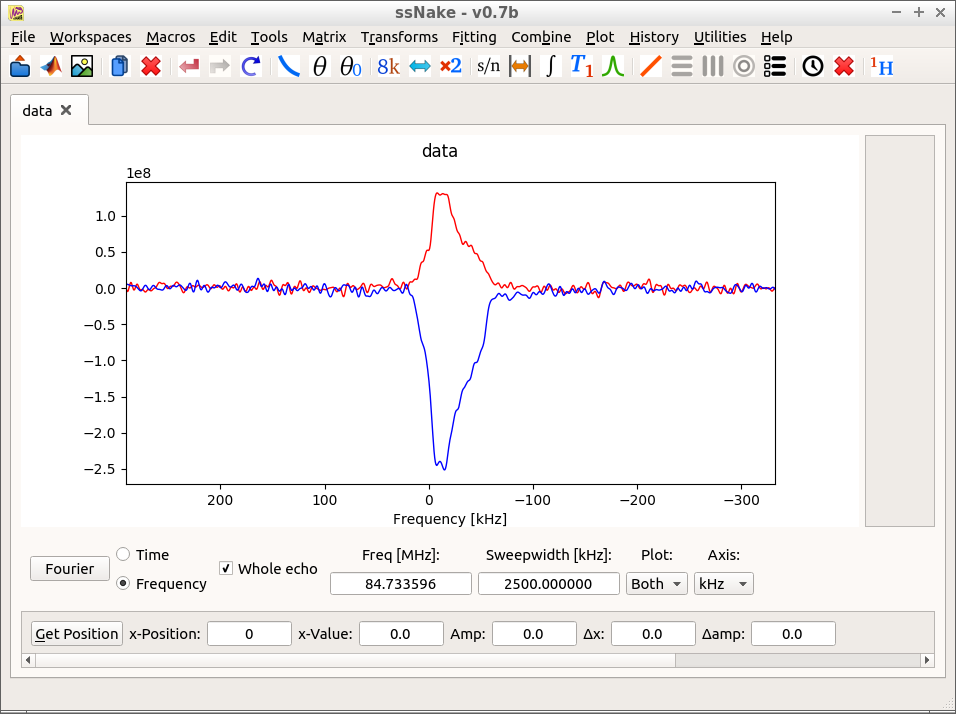
\includegraphics[width=0.8\linewidth]{Figs/Fig3.png}
\end{center}

To get the desired spectrum, we now need to phase it to make the imaginary part zero, and the real part positive:
\begin{itemize}
\item Phase with -152$^\circ$ zero order order phasing (`Tools $\longrightarrow$ Phasing')
\end{itemize}
This gives the final spectrum:
\begin{center}
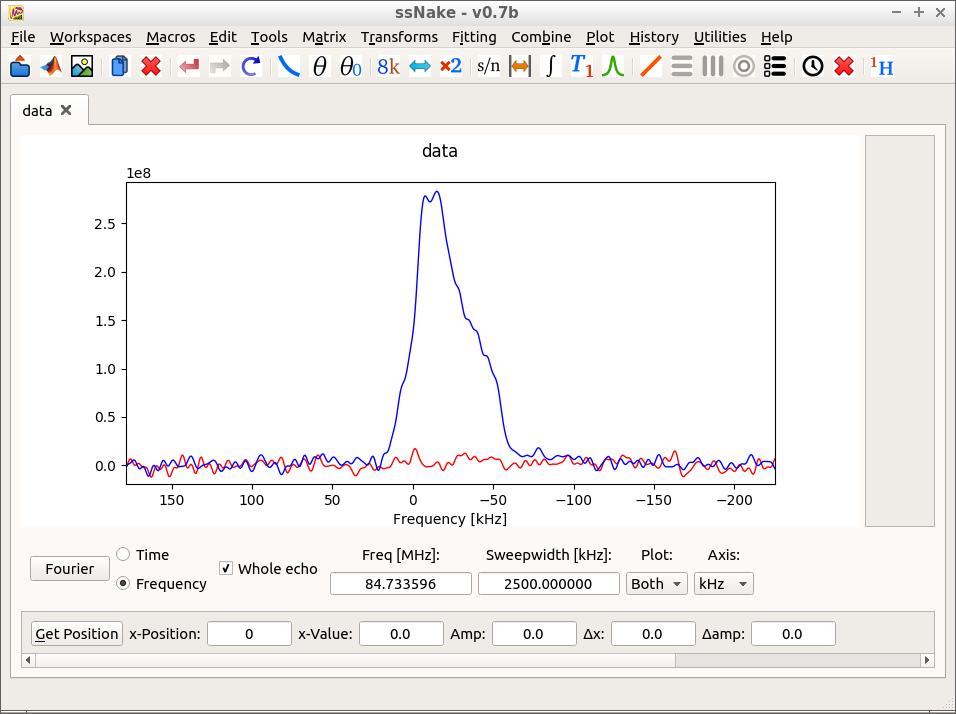
\includegraphics[width=0.8\linewidth]{Figs/Fig4.png}
\end{center}

Optionally, you can now fit this 2nd order quadrupolar lineshape via `Fitting $\longrightarrow$
Quadrupole'. This will lead to C$_\text{Q}$ = 15.6 MHz, and $\etaup = 0.78$. Do remember that $^{139}$La has a spin quantum number of 7/2.

\section{Alternatives}
\subsection{Wrong echo top}
In some cases, the echo top of the data is hard to establish. When the echo is split at the wrong part, a first order phasing is introduced in the spectrum, and zero order phasing only will still lead to some imaginary component. If the echo is swapped at index 461, the following zero order phased (-154.7$^\circ$) spectrum is found:
\begin{center}
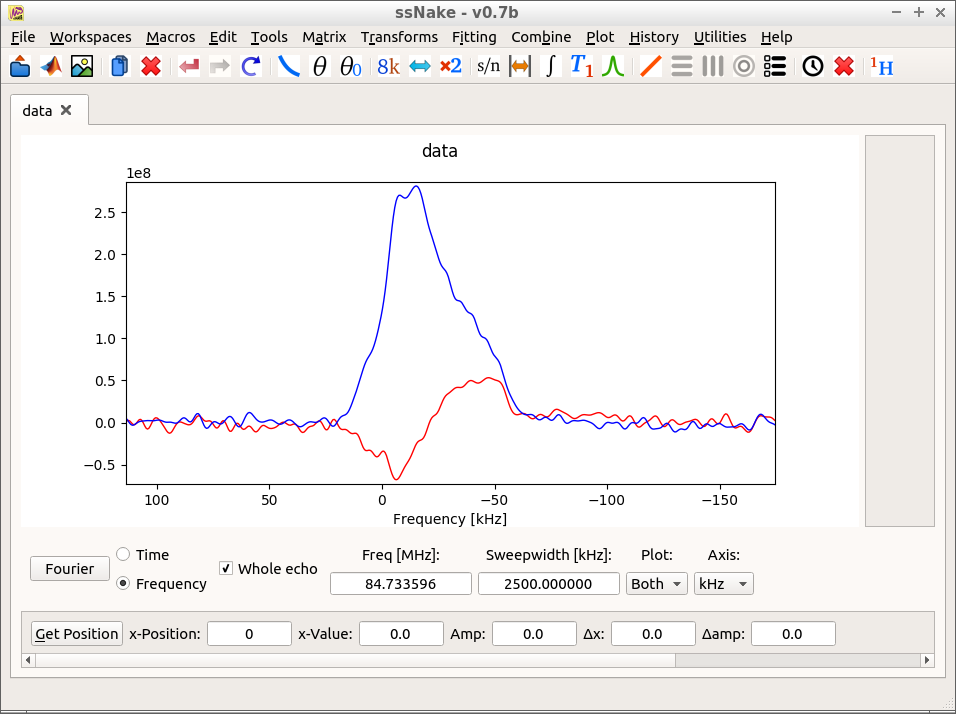
\includegraphics[width=0.8\linewidth]{Figs/Fig5.png}
\end{center}

This can be fixed using a first order phasing. After first order phasing (2332$^\circ$ at reference -20317) the properly phased spectrum is recovered:
\begin{center}
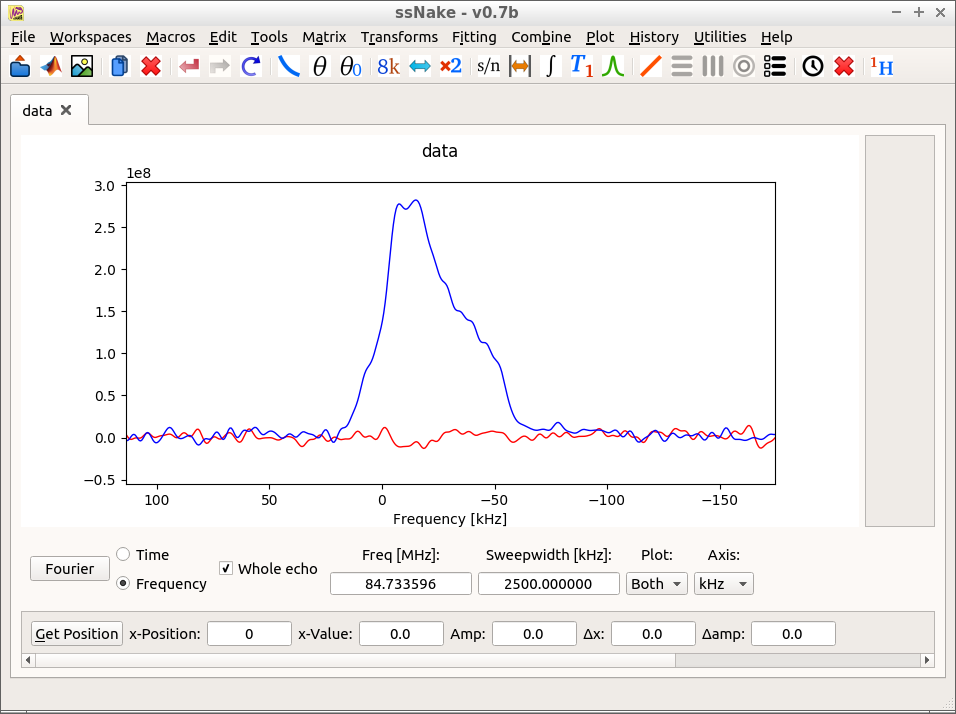
\includegraphics[width=0.8\linewidth]{Figs/Fig6.png}
\end{center}




\end{document}
